Una vez calculada la ganancia del SiPM a partir de los  datos, procedemos a determinar la dependencia  del SiPM con la temperatura. En concreto, nos interesa determinar el comportamiento de su ganancia cuando varía la temperatura. Para ello realizamos una serie de medidas a distintas temperaturas y, para cada una de ellas, calculamos la ganancia a partir del método expuesto en el apartado anterior.

Nos centraremos en el intervalo de temperatura entre $15~\celsius$, que es el mínimo al que nos permitía llegar el sistema de control de temperatura y $41~\celsius$, que, suponemos, es el límite al que llegará nuestro futuro detector en la práctica. Es decir, este intervalo de temperaturas es equivalente a las temperaturas a las que estará sometido nuestro detector debido a las condiciones climáticas del lugar. Realizaremos pasos de $2~\celsius$ entre cada medida realizando un total de $14$ medidas. Realizaremos medidas de  $15000$ eventos  que son suficientes para obtener un espectro  suave. 

Para automatizar este proceso, hemos desarrollado una macro en ROOT que realice este ajuste. Esta macro se divide en dos partes:
\begin{itemize}
\item{} Por un lado,  posee un bucle en el que, en cada paso, abre el fichero correspondiente a una temperatura, empezando por la mínima ($15~\celsius$) realiza todo el estudio anterior y guarda ganancia y temperatura con sus errores en 4 vectores respectivamente. En cada paso aumenta $2~\celsius$ la temperatura y pasa a leer el siguiente fichero.
Hay que tener en cuenta que, como se dijo anteriormente, el sistema de control de temperatura debe de estar en la zona uno del diagrama de fases existente en la ficha técnica. Esto implica que, para medidas inferiores a $27~\celsius$ necesitamos aumentar la humedad en un $5\%$ en cada medida (humedad del $45\%$ para $25~\celsius$, $50\%$ para $23~\celsius$, etc.). Esto no tiene mayor importancia, ya que se vio que la ganancia del SiPM no se ve afectada de forma apreciable ante modificaciones de la humedad de este tamaño.
La incertidumbre en la temperatura viene dada por la oscilación en el valor de la temperatura observada directamente en el panel de control del sistema. La oscilación observada fue en todo momento de $0.1~\celsius$, una incertidumbre totalmente inapreciable tanto a nivel visual en la gráfica como a nivel de variación de la ganancia.

\item {} Por otro lado, partiendo de estos $4$ vectores de dimensión $14$ en nuestro caso (igual al número de ficheros que ha leido) que contienen ganancia, temperatura y sus errores de forma ordenada la macro realiza un ajuste lineal. El ajuste obtenido se presenta en la figura~\ref{temperatura}.

\begin{figure}[hbtp]
\centering
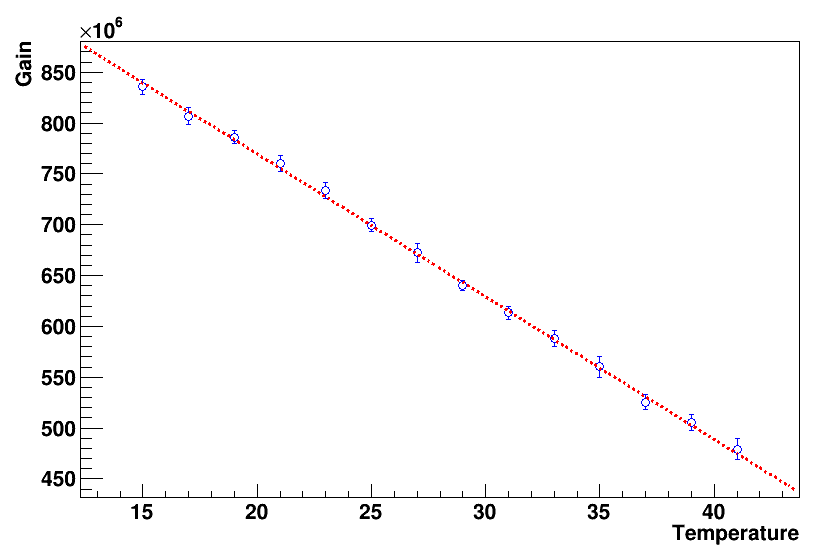
\includegraphics[scale=0.4]{Dependenciatemperatura.png}
\caption{ Ganancia frente a temperatura\label{temperatura}}
\end{figure}

Podemos observar la existencia de un comportamiento lineal casi perfecto en un intervalo de temperatura de $26~\celsius$. Esta es una propiedad que caracteriza al SiPM, una muy buena linealidad en su comportamiento frente a modificaciones en varias magnitudes. Nuevamente comprobamos la calidad del ajuste a partir del test $\chi^2$ obteniendo un valor de $\frac{\chi^2}{ndf}=\frac{2.937}{12}\approx 0.245$, que es un valor relativamente bueno.

En la gráfica~\ref{temperatura} encontramos, como esperábamos~\cite{tesisSiPM}, la existencia de un decrecimiento del valor de la ganancia del SiPM a medida que aumenta la temperatura. Esto es debido a que la zona desierta, que se crea en el SiPM al aplicar un voltaje en inversa y que actúa como zona útil de detección de radiación, depende de la temperatura. En concreto, al aumentar la temperatura estamos incrementando la excitación térmica de los portadores de carga pudiendo, de esta forma, invadir esta zona desierta, reduciéndola su tamaño y, por extensión, la ganancia del SiPM.

La ecuación obtenida en este ajuste $G=aT+b$ toma los siguientes valores: 
\begin{equation}
a=(-140.3 \pm 2.7) \cdot 10^5~\frac{1}{\celsius}
\label{ajustependientetemperatura}
\end{equation}
\begin{equation}
b=(1050.0 \pm 7.7) \cdot 10^6
\label{ajusteordenadatemperatura}
\end{equation}


Esta es un resultado importante, no por el valor numérico, sino porque será la base que utilizaremos para conseguir la compensación de la ganancia.
\end{itemize}